
\begin{figure}[t]
    %\hspace{-10pt}
    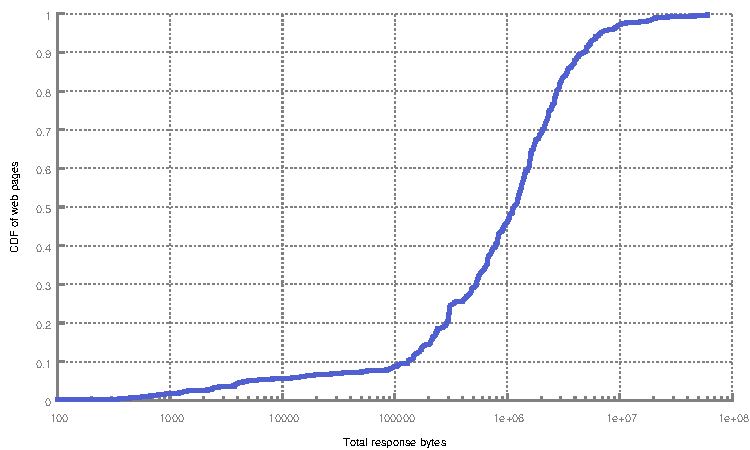
\includegraphics[width=3.25in]{../graphs/total_bytes/total_bytes.pdf}
    \caption[]{\label{fig:total_bytes} Total Bytes. Log Scale.}
\end{figure}

%\begin{figure}[t]
%    %\hspace{-10pt}
%    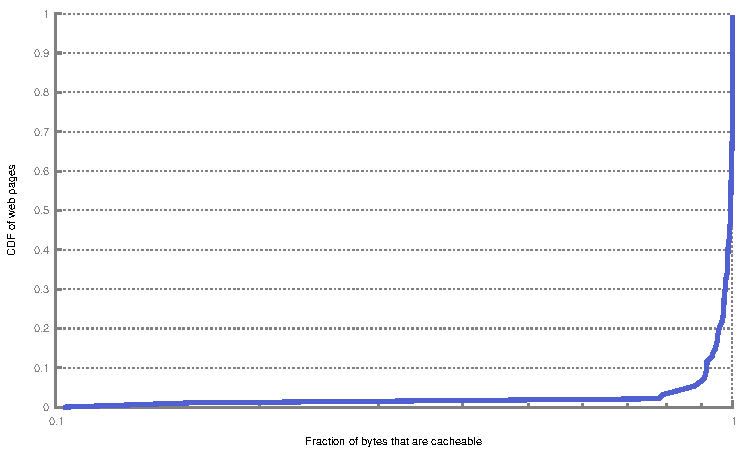
\includegraphics[width=3.25in]{../graphs/cacheable_bytes/cacheable_bytes.pdf}
%    \caption[]{\label{fig:cacheable_bytes} Cacheable Bytes. Log scale}
%\end{figure}

\begin{figure}[t]
    %\hspace{-10pt}
    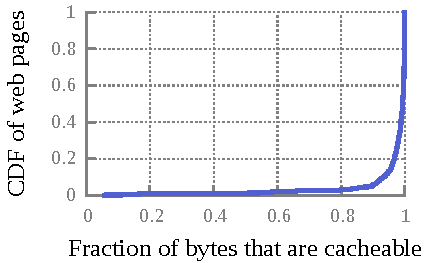
\includegraphics[width=3.25in]{../graphs/cacheable_bytes/cacheable_bytes_linear.pdf}
    \caption[]{\label{fig:cacheable_bytes_linear} Cacheable Bytes. Linear
    Scale.}
\end{figure}

\begin{figure}[t]
    %\hspace{-10pt}
    \includegraphics[width=3.25in]{../graphs/plts/plts.pdf}
    \caption[]{\label{fig:plts} Page Load Times. Linear
    Scale.}
\end{figure}

%\begin{figure}[t]
%    %\hspace{-10pt}
%    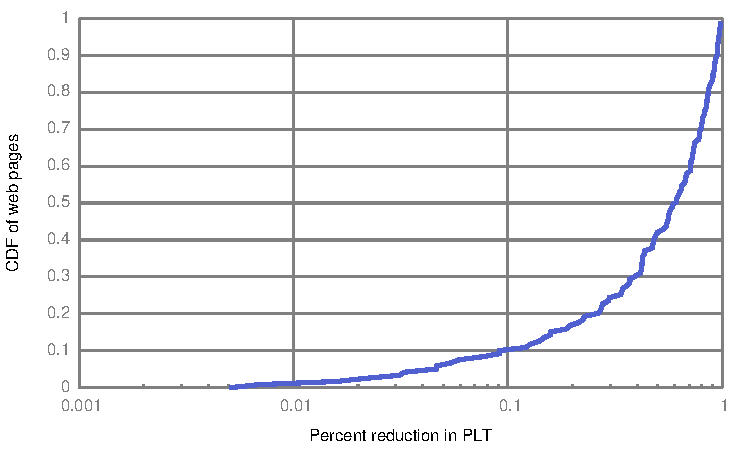
\includegraphics[width=3.25in]{../graphs/percent_plt_reduction/percent_reduction.pdf}
%    \caption[]{\label{fig:percent_reduction} Fraction Reduction. Log Scale.}
%\end{figure}

\begin{figure}[t]
    %\hspace{-10pt}
    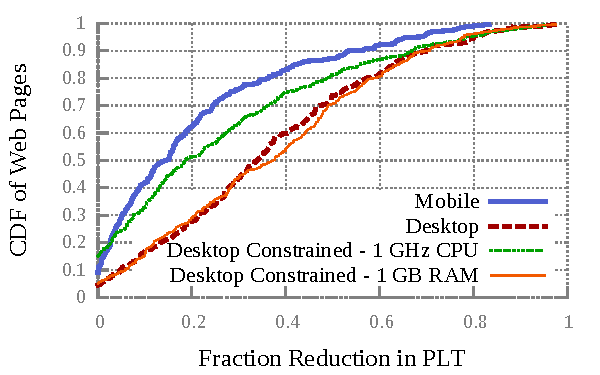
\includegraphics[width=3.25in]{../graphs/percent_plt_reduction/percent_reduction_linear.pdf}
    \caption[]{\label{fig:percent_reduction_linear} Fraction Reduction. Linear Scale.}
\end{figure}

\begin{figure}[t]
    %\hspace{-10pt}
    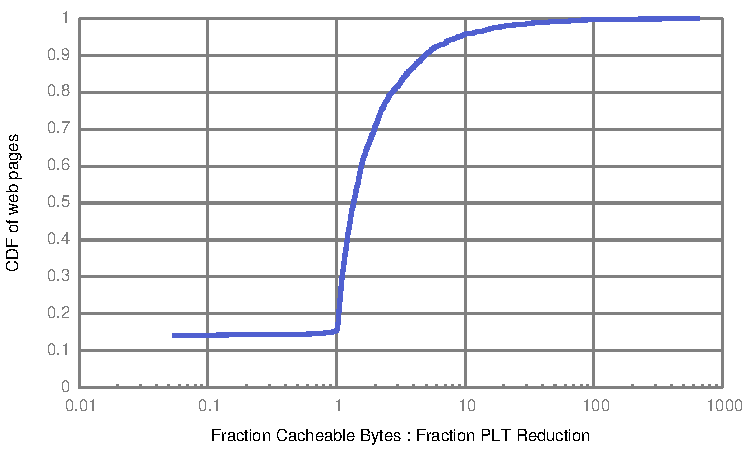
\includegraphics[width=3.25in]{../graphs/ratio_bytes_to_reduction/ratio.pdf}
    \caption[]{\label{fig:ratio} Fraction Cacheable Bytes : Fraction PLT
    Reduction. Log Scale.}
\end{figure}

\begin{figure}[t]
    %\hspace{-10pt}
    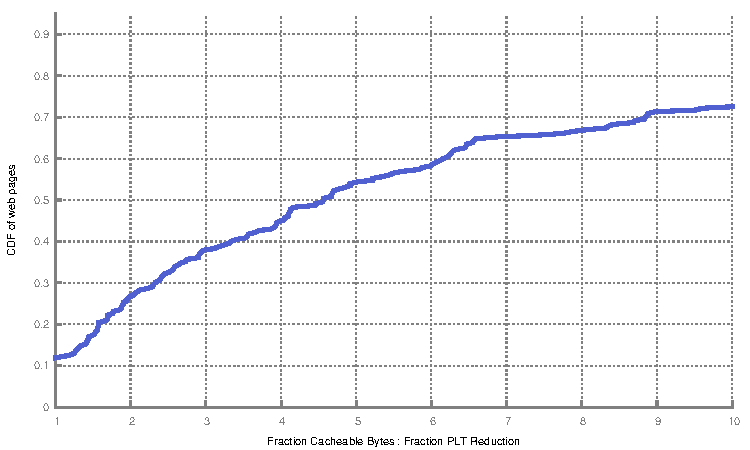
\includegraphics[width=3.25in]{../graphs/ratio_bytes_to_reduction/ratio_linear.pdf}
    \caption[]{\label{fig:ratio_linear} Fraction Cacheable Bytes : Fraction PLT
    Reduction. Linear scale, with datapoints past 95th percentile, and below
    X=1 cut off.}
\end{figure}

\begin{figure}[t]
    %\hspace{-10pt}
    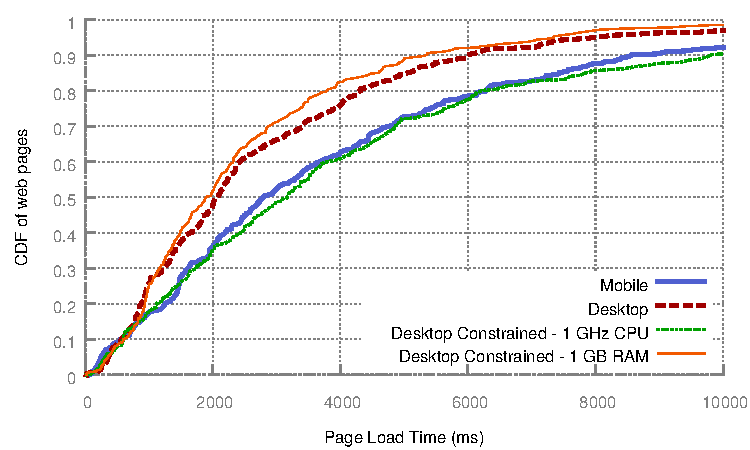
\includegraphics[width=3.25in]{../graphs/plt_comparison/plt_differences.pdf}
    \caption[]{\label{fig:plt_comparison} Sanity check: differences between
    PLTs.}
\end{figure}

Figure~\ref{fig:ratio} is the most interesting, and requires some pondering.
Datapoints to the left of X=1 indicate that caching yielded a large
bang for its buck, i.e. fraction speedup from perfect caching was greater than fraction of
cacheable bytes. This is about 8\% of the pages. I suspect that this is
largely due to
variation in performance.

At X=1, we see roughly 10\% of pages had PLT improvements commensurate with
fraction of cached byes.

Then right of X=1, the remaining 70ish\% of pages showed that ``a buck's worth
of cache hits amounts to less than a buck's worth of PLT improvement''. It's
hard to see on the logarithmic axis just how many cents of PLT a buck worth of
caching buys. Figure~\ref{fig:ratio_linear} shows us that it's around 75 cents
to the dollar for the 20th through the 70th percentiles. After that, the
payoff starts decreasing rapidly (below 50 cents) for the remaining 40 percentiles.
